
The workflow is depicted in Figure \ref{fig:protocol}, and described with full details as follows.

\begin{figure}[h]
	\centering
		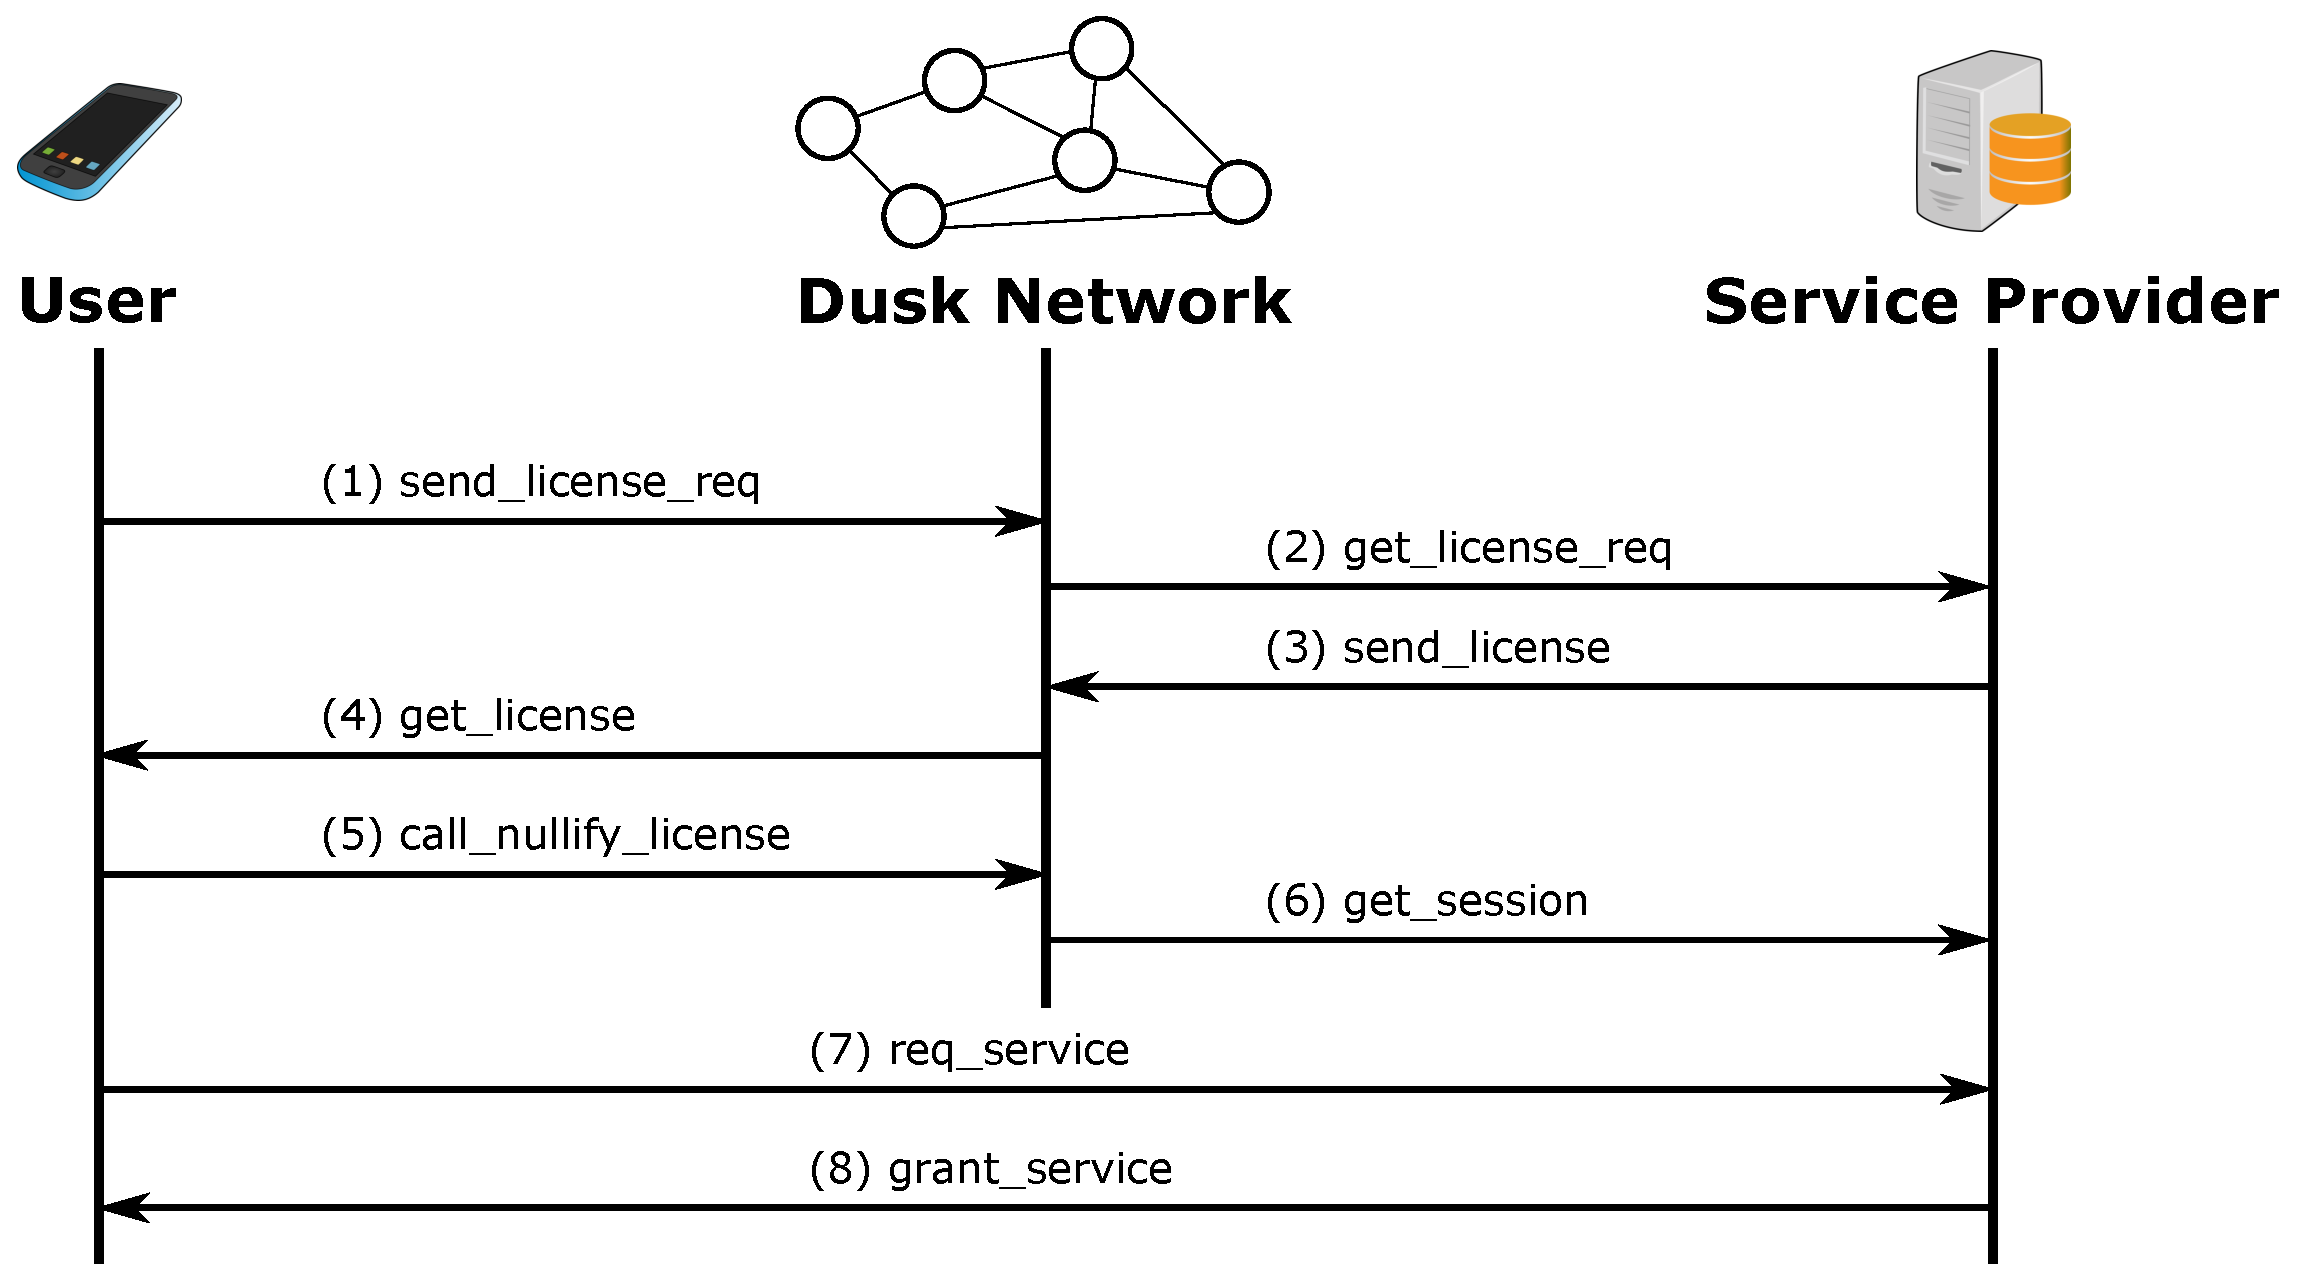
\includegraphics[width=390pt,draft=false]{images/protocol.eps}
	\caption{Overview of the protocol messages exchanged between the user, the Dusk Network, and the SP.}
	\label{fig:protocol}
\end{figure}

\begin{enumerate}
	\item (\textbf{user}) $\mathsf{send\_license\_req}$ : compute a license stealth address $(\lpk, R)$ belonging to the user, using the user's own public key, and also an additional key $\ksym_{\License} = \hb(\lsk)G$, by computing first the user's $\lsk$. Then, compute the request stealth address $(\rpk, R)$ and $\kdh$ using the SP's public key. And finally send the following request to the network:


		$$\Request = ((\rpk, R), \enc, \nonce)$$,

	where 

		$$\enc = \Enc_{\kdh} ((\lpk, R)||\ksym_{\License}; \nonce)$$.


	\item (\textbf{SP}) $\mathsf{get\_license\_req}$ : continuously check the network for incoming license requests.

	\item (\textbf{SP}) $\mathsf{send\_license}$ : upon receiving a request from a user, define a set of attributes $\attr$ representing the license, and compute a digital signature as follows:

		$$\lsig = \sign_{\sk_{\SP}}(\lpk, \attr)$$.

	Then, send the following license to the network:

		$$\License = ((\lpk, R), \enc, \nonce, \pos)$$,

	where 

		$$\enc = \Enc_{\ksym_{\License}} (\lsig || \attr; \nonce)$$.

	\item (\textbf{user}) $\mathsf{get\_license}$ : receive the license by scanning the incoming transactions.

	\item (\textbf{user}) $\mathsf{call\_nullify\_license}$ : when desiring to use the license, nullify it by executing a call to the license contract. The following steps are performed:

	\begin{itemize}
		\item The user issues a transaction that calls the license contract, which includes a ZKP that is computed out of the gadget depicted in Figure \ref{fig:circuit_prove_nft}.
		\item The network validators will execute the smart contract, which verifies the proof. Upon success, the following session will be added to a shared list of sessions:

			$$\Session = \{\mathsf{session\_hash}, \lnullifier, \com_0^{hash}, \com_1, \com_2\}$$,

		where $\mathsf{session\_hash} = \hp(\pk_{\mathsf{SSP}} || \mathsf{r})$.


	\end{itemize}

	\item (\textbf{user}) $\mathsf{req\_service}$ : request the service to the SSP, establishing communication using a secure channel, and providing the $\SessionCookie$.

	\item (\textbf{SSP}) $\mathsf{get\_session}$ : receive a $\Session$ from the list of sessions, where $\Session.\lnullifier = \SessionCookie.\lnullifier$.

	\item (\textbf{SSP}) $\mathsf{grant\_service}$ : grant or deny the service upon verification of the following steps:

	\begin{itemize}
		\item Check whether the values $(\attr, \pk_{\SP}, c)$ included in the $\SessionCookie$ are correct.
		\item Check whether the opening $(\pk_{\mathsf{SSP}}, \mathsf{r})$ included in the $\SessionCookie$ matches the $\mathsf{session\_hash}$ found in the $\Session$.
		\item Check whether the openings $((\pk_{\SP}, \mathsf{s_0}), (\attr, \mathsf{s_1}), (c, \mathsf{s_2}))$ included in the $\SessionCookie$ match the commitments ($\com_0^{hash}, \com_1, \com_2$) found in the $\Session$.
	\end{itemize}

\end{enumerate}

\begin{figure}[h]
	\centering
	\setlength{\fboxsep}{5pt}%
	\setlength{\fboxrule}{0.3pt}%
	\fbox{
		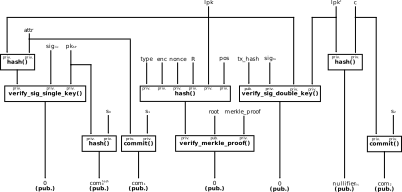
\includegraphics[width=460pt,draft=false]{images/circuit_prove_nft.eps}}
	\caption{Arithmetic circuit for proving a license's ownership.}
	\label{fig:circuit_prove_nft}
\end{figure}

Furthermore, the SSP might request the user to nullify the license they are using (e.g. this is a single-use license, like entering a concert). This is done through the computation of $\lnullifier$. The deployment of this part of the circuit has two different possibilities:
\begin{itemize}
	\item If we set $c = 0$ (or directly remove this input from the circuit), the license can be used only once.
	\item If the SSP requests the user to set a custom value for $c$ (e.g. the date of an event), the license can be reused only under certain conditions.
\end{itemize}
